\documentclass{minimal}
\usepackage{lscape}
\usepackage{tikz}

\begin{document}
\begin{landscape}
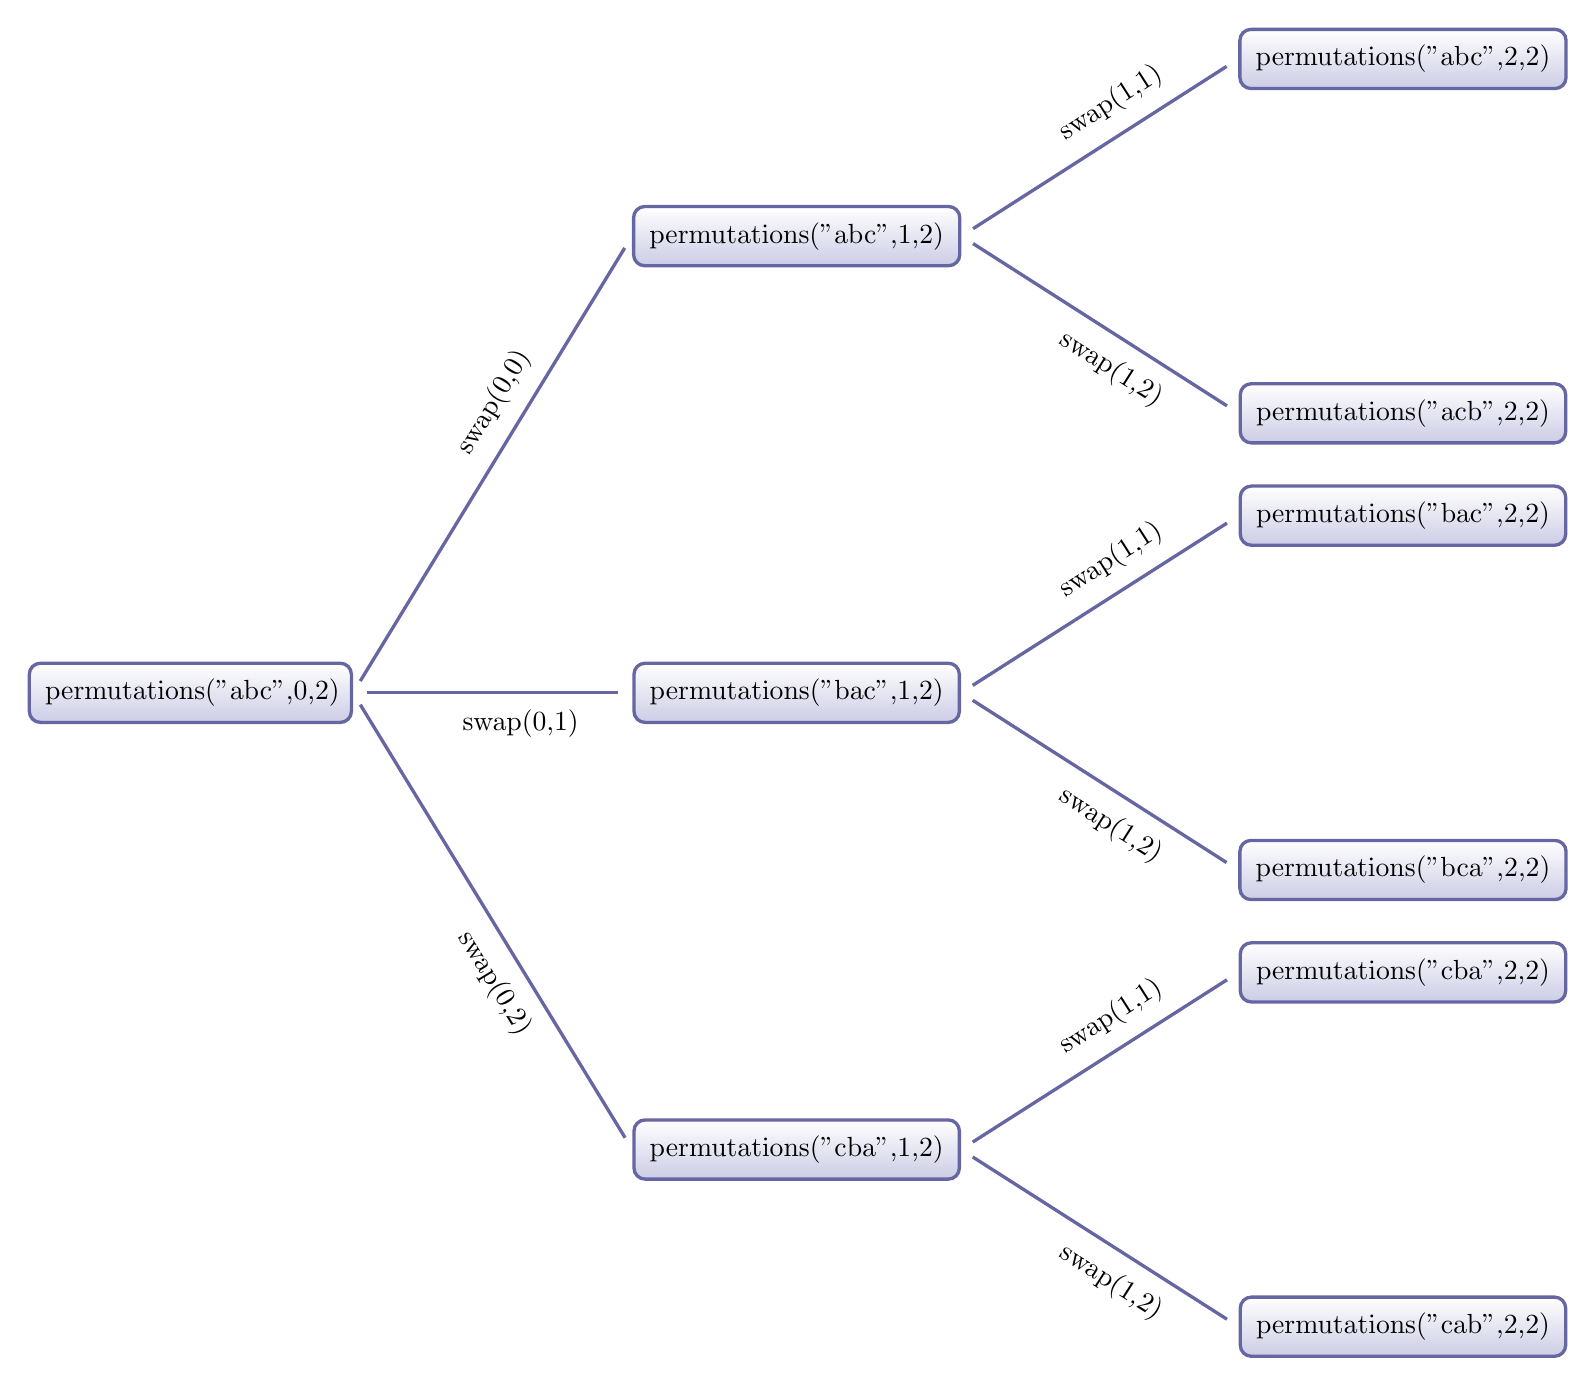
\begin{tikzpicture}
   [
    grow=right,
    level 1/.style={sibling distance=5.8cm,level distance=7.7cm},
    level 2/.style={sibling distance=4.5cm,level distance=7.7cm},
    edge from parent/.style={very thick,draw=blue!40!black!60,
                             shorten >=5pt, shorten <=5pt},
    edge from parent path={(\tikzparentnode.east) --(\tikzchildnode.west)},
    kant/.style={text width=2cm, text centered, sloped},
    every node/.style={text ragged, inner sep=2mm},
    punkt/.style={rectangle, rounded corners, shade, top color=white,
    bottom color=blue!50!black!20, draw=blue!40!black!60, very
    thick }
    ]

\node[punkt, text width=10.5em] {permutations("abc",0,2)}
    %lv1 child1
    child {
      node[punkt]{permutations("cba",1,2)}
           % lv2 child 1
           child{
             node[punkt][text ragged]{permutations("cab",2,2)}
                 edge from parent 
                 node[kant, below, pos=.6] {swap(1,2)}
           }
           % lv2 child 2
           child{
             node[punkt][text ragged]{permutations("cba",2,2)}
                  edge from parent
                  node[kant, above, pos=.6] {swap(1,1)}
           }
    edge from parent
    node[kant, below, pos=.6] {swap(0,2)}
    }
    %lv1 child2
    child {
      node[punkt][text ragged]{permutations("bac",1,2)}
           % lv2 child 1
           child{
             node[punkt][text ragged]{permutations("bca",2,2)}
                 edge from parent 
                 node[kant, below, pos=.6] {swap(1,2)}
           }
           % lv2 child 2
           child{
             node[punkt][text ragged]{permutations("bac",2,2)}
                  edge from parent
                  node[kant, above, pos=.6] {swap(1,1)}
           }
    edge from parent
    node[kant, below, pos=.6] {swap(0,1)}
    }
    %lv1 child3
    child {
      node[punkt][text ragged]{permutations("abc",1,2)}
           % lv2 child 1
           child{
             node[punkt][text ragged]{permutations("acb",2,2)}
                 edge from parent 
                 node[kant, below, pos=.6] {swap(1,2)}
           }
           % lv2 child 2
           child{
             node[punkt][text ragged]{permutations("abc",2,2)}
                  edge from parent
                  node[kant, above, pos=.6] {swap(1,1)}
           }
    edge from parent
    node[kant, above, pos=.6] {swap(0,0)}
    };
   
    
\end{tikzpicture}
\end{landscape}
\end{document}
